% !TeX root = ../Book1.tex
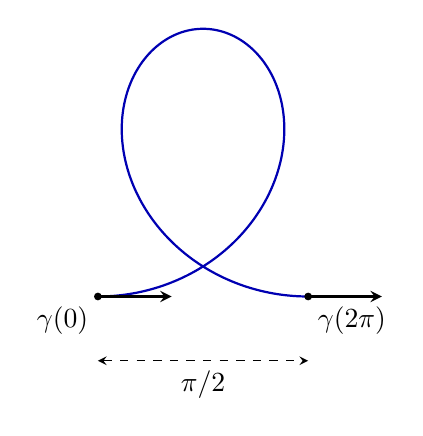
\begin{tikzpicture}[x=1.7cm,y=1.7cm,>=stealth]
	\draw[blue!70!black,thick,domain=0:360,samples=161,smooth,variable=\t] plot ({sin(\t)+0.5*(\t*pi/360+sin(2*\t)/4)},{1-cos(\t)+0.25*sin(\t)^2});
	\fill (0,0) circle (1.4pt) node[below left] {\(\gamma(0)\)};
	\fill ({pi/2},0) circle (1.4pt) node[below right] {\(\gamma(2\pi)\)};
	\draw[->,thick] (0,0)--(0.55,0);
	\draw[->,thick] ({pi/2},0)--({pi/2+0.55},0);
	\draw[<->,dashed] (0,-0.48)--node[below] {\(\pi/2\)} ({pi/2},-0.48);
\end{tikzpicture}
